\chapter{Motivation}

Im Folgenden wird die Motivation für diese Arbeit, sowie die Relevanz dieser Arbeit in dem Kontext des \textit{\ac{SCP}} dargelegt. Dafür erfolgt zunächst eine kurze Einführung in \ac{SCP} bei SAP und in konkret eine Methode, die angewandt wird, um Rechenzeit zu reduzieren. Daraufhin wird ein Problem bei diesem Verfahren vorgestellt und schließlich die Ziele und das geplante Vorgehen für diese Arbeit diskutiert.

\section{SAP Supply Chain Optimizer} \label{sec:sap_scp}

Das \textit{\ac{SCP}} stellt für viele Unternehmen in einer globalisierten, digitalisierenden Welt mit sich immer schneller verändernden Märkten eine zunehmende Herausforderung dar.n Optimierungslauf wird von den Kunden zumeist  einmal täglich durchgeführt.

\section{Product Decomposition und Similarity} \label{sec:proddeco}

Für besonders große Szenarien kann es wünschenswert oder sogar nötig werden die Komplexität des Szenarios zu reduzieren, um mit geringerem Ressourcenaufwand in Form von Laufzeit und Speicher eine optimierte Lösung   nach \autoref{sec:sap_scp} zu erhalten. Dies kann zum Beispiel mit der \textit{\ac{ProdDeco}} bewerkstelligt werden \cite{.20220812}. Hierfür wird die gesamte Supply Chain in jeweils kleinere \textit{Subprobleme} aufgeteilt. Diese stellen Gruppen aus Produkten dar, die möglichst wenig Berührungspunkte mit anderen Subproblemproduktgruppen haben. Die Subprobleme werden dann individuell und unabhängig voneinander optimiert~\cite[S.~31--33]{Sandner.01.09.1998}.   

In \autoref{fig:sim_alg} ist die Synthese der Subprobleme mithilfe der Similarity illustriert. Dieser Vorgang wiederholt sich bis alle Submodelle zu Subproblemen zugeordnet worden sind (6). \\ %macht zeilenumbruch
Wenn $n$ die Anzahl an atomaren Submodellen ist, folgt direkt aus dem Algorithmus per Gaußscher Summenformel
\begin{align}
\label{eq:num_comp} \#S := \sum_{i=0}^{n} i = \frac{n(n+1)}{2} \in O(n^2)
\end{align}
für die Anzahl der paarweisen Vergleiche und damit die Anzahl der Similarity-Berechnungen $\#S$. \\
Für die Zeitkomplexität der Subproblemsynthese $t_{sub}$ gilt also \autoref{eq:t_sim}, wobei $m$ die durchschnittliche Größe - also die durchschnittliche Anzahl der Elemente - der Submodelle beschreibt.
\begin{align}
	\label{eq:t_sim} t_{sub}(n, m) \in O(\#S \cdot t_{sim}(m)) = O(n^2 \cdot t_{sim}(m)) 
\end{align}

\begin{figure}
	\centering
	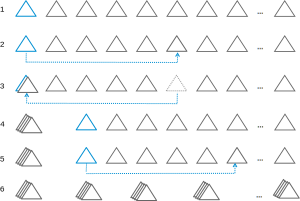
\includegraphics[width=0.80\textwidth]{Bilder/similarity_algorithm.pdf} 
	\caption{Abstrakter Synthesealgorithmus der Subprobleme unter Nutzung der Ähnlichkeit der Submodelle. \\ (In Anlehnung an \cite{Kniasew.21.02.2022}.)}
	\label{fig:sim_alg}
\end{figure} 

\section{Problemszenario} \label{sec:problem}

Als Übergangslösung wurde der Algorithmus für das kritische Szenario so angepasst, dass eine Menge Informationen außer acht gelassen wurden, um auf Kosten der Lösungsqualität eine akzeptable Laufzeit von $14 min$ $47 s$\footnote{Zeit von lokalem Testsystem (s. \autoref{sec:perf})} zu erreichen. \\
Die Supply Chain des Ausgangsszenarios hat hierbei insgesamt ca. 1.97 Mio. Elemente und die 18771 erstellten atomaren Submodelle im Mittel jeweils ca. 5100 Elemente \cite{Kniasew.21.02.2022}. 

Das bedeutet nach \autoref{eq:num_comp} bereits $\#S = \frac{18771 \cdot (18771 + 1)} {2} \approx 176'000'000$ Vergleiche die durchgeführt werden müssen. Für den Worst-Case ist  $t_{sim}$ mit $t_{sim}(m) \in O(m \log m)$\footnote{Auf die Unterscheidung zw. $m_{1}$ und $m_{2}$ wird hier aufgrund des $O$-Kalküls und der Verwendung von $m$ als Mittelwert der Elementzahlen verzichtet.} angegeben \cite{Kniasew.21.02.2022}. Für $m=5100$ ergeben sich die asymptotischen Ungleichungen 
\begin{align}
	t_{sim}(m) \preccurlyeq m \log m \approx 62800 \implies \nonumber \\
	\label{eq:conrete_id_obj} t_{sub}(n, m) \preccurlyeq \#S \cdot m \log m \approx 176'000'000 \cdot 62800 \approx 11 \cdot 10^{12}
\end{align}


\section{Zielsetzung, Inhalt und Vorgehensweise}

Es ist ersichtlich, dass Anlass zur Verbesserung der Laufzeit gegeben ist, um 
\begin{enumerate}
\item das kritische Szenario ohne Weglassen von Informationen durchführbar zu machen und
\item die durchschnittlichen Szenarien zu verbessern, um Rechenzeit und damit langfristig Energie zu sparen.  
\end{enumerate}  
Hierfür wird sich vor allem auf $t_{sim}$ und dessen Minimierung fokussiert. Ziel ist es, eine neue Art der Similarity-Berechnung zu finden, die schneller abläuft als die alte, aber dabei noch die genau gleichen Subprobleme erzeugt. 